%\part{Mantendo Suas Moedas Seguras}
\chapter{Protegendo o livro-razão}
\label{ch:capitulo6}
%\setcounter{chapter}{5}
Até agora, falamos como gerenciamos e mantemos as cópias e gravamos no livro-razão distribuído sem que possa haver coerção ou corrupção, utilizando um sistema de loteria e a validação por consenso.

Mas o que acontece quando um ganhador da loteria quer ser malicioso? Ganhar o direito de escrever em livro-razão significa que eles podem alterar lançamentos históricos no livro-razão? Evandro, Danilo e Fernanda podem conspirar para reescrever a história ou alterar os saldos das contas e dar a si mesmos moedas extras?

Ai vem a \textit{blockchain}. Um termo de marketing que permeou grande parte do setor de tecnologia, a blockchain nada mais é do que a ideia de que os \textit{blocos} do Bitcoin são \textit{encadeados} para fornecer links de um conjunto de transações para o próximo bloco.
Isso cria uma registro histórico linear de cada bloco desde o bloco gênesis extraído por Satoshi em 2009 ate hoje.

Mentimos um pouco no capítulo anterior para manter as coisas mais simples.
Quando você minera jogando na loteria de Prova de Trabalho, você não está apenas fazendo o hash das transações que querem ir para o próximo bloco junto com o nonce.
Na verdade, você também está fornecendo o hash do último bloco como entrada em sua função hash, vinculando assim seu bloco ao bloco anterior.

%\newpage



%nao tem essa figura no meu livro

% \begin{figure}
%   \centering
%   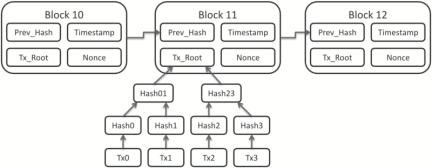
\includegraphics[width=10cm]{imagens/capitulo-06-bloco.jpg}
%   \caption{\url{https://upload.wikimedia.org/wikipedia/commons/7/7a/Bitcoin_Block_Data.png}}
% \end{figure}

Lembre-se de que a saída de uma função hash é aleatória e dependente de todos os dados de entrada que nela constam. 
Agora modificamos nossos hashes do bloco para incluir três entradas diferentes:

\begin{samepage}
\begin{enumerate}
\item As transações que queremos incluir no livro-razão;
\item Um nonce aleatório;
\item O hash do bloco anterior que estamos usando como sendo a base do histórico do livro-razão.
\end{enumerate}
\end{samepage}

\begin{figure}[ht]
  \centering
  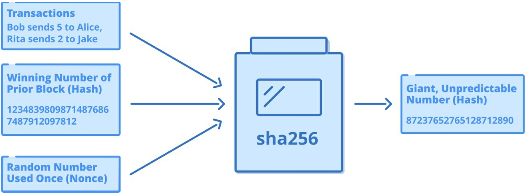
\includegraphics[width=10cm]{imagens/capitulo6/capitulo6Sha256.png}
  \caption*{\textit{\small As três entradas usadas para construir o hash para participar da loteria, agora incluindo o hash ganhador anterior, fazendo um cadeia entre um bloco e outro.}}
\end{figure}

Isso nos permite construir um registro histórico de cada bloco desde o Bloco gênesis (primeiro bloco do Bitcoin) extraído por Satoshi.
Quando escrevemos um novo bloco na blockchain, temos que validar que este bloco não contém nenhuma transação que gaste bitcoins que já foram gastos em blocos anteriores.

Se alguma dessas três entradas forem alteradas, o hash de saída mudará drasticamente e de maneira imprevisível. Esse comportamento cria uma propriedade interessante: se você adulterar os dados de qualquer bloco antigo, alterará seu hash. Se você alterar o hash de qualquer bloco antigo, alterará o hash de cada bloco que vier depois, atuando como uma especie de foto de toda a historia da rede ate esse ponto!

%nao Possui essa frase ate entao.
%Isso torna a corrente inviolável. Se alguém tentasse alterar um bloco mais antigo na cadeia, teria que recalcular o hash de Prova de Trabalho do bloco que está adulterando e de cada novo bloco que vier depois.

Você não pode adulterá a prova de trabalho, como todos sabem a quantidade de energia que precisa ser gasta em cada bloco baseado no numero alvo para esse bloco. Se alguém for tentar mudar um bloco mais velho, eles precisariam computar o hash de prova de trabalho daquele bloco e de todos os bloco que vieram depois. Não só a blockchain deixa adulterações evidentes, como ela torna extremamente caro realizar a adulteração.

Efetivamente, cada novo bloco minerado no Bitcoin aumenta a segurança dos blocos que vieram antes dele, por conta do aumento da quantidade de energia necessária para recalcular todos os hashes para modificar um ponto anterior da rede.
%adicionando acima 
Uma transação em um bloco que possui 6 blocos posteriores a ele é considerada definitivamente inalterada. 
Seria necessária uma enorme quantidade de energia para recalcular os últimos seis blocos na taxa de hash total atual.
Alterar um bloco a 100 blocos atrás? Nem pense nisso, esquece.

%adicionado
Quando fazes o download de uma copia da \textit{blockchain}  todas as transições são completamente transparentes e você pode verificar os hashes da prova de trabalho para garantir que nada foi alterado por alguém que lhe enviou o livro-razão.


%when blocks colilde( Troquei de posição pois na minha versao ele acontece aqui) 
%%
\section*{Quando Blocos Collidem}%E se duas pessoas encontrarem um bloqueio ao mesmo tempo?}


Falta uma peça no sistema de consenso. 
Como podemos forças todos a utilizar a mesmo histórico das transações se ocorrer o caso de dois mineradores simultaneamente minerar dois blocos e anunciam eles a rede?

Imagine que agora estamos administrando uma rede mundial. Pessoas em todo o mundo, dos Brasil ao Japão, estão conectadas a essa rede global e todas estão jogando na loteria da Prova de Trabalho.

Alguém em São Paulo encontra um bloco válido. Eles o anunciam na rede e todos os computadores do Brasil começam a detectá-lo. Enquanto isso, alguém em Tókio também encontra um bloco a poucos segundos depois do bloco de São Paulo. Seus vizinhos ainda não ouviram falar do bloco brasileiro, então eles ficam sabendo primeiramente do bloco japonês.

%adicionado
Ambos os blocos contem uma transação de 1 bitcoin de Ana a \TraducaoNomeB. Mas logo na sequencia \TraducaoNomeB{} envia o bitcoin para \TraducaoNomeC. Devido a diferença de tempo o bloco brasileiro o próximo bloco brasileiro vai refletir essa transação e o \TraducaoNomeB{} vai ter um saldo na conta de zero. Entretanto, o bloco japonês minerou seu bloco antes de ver a transação de \TraducaoNomeB{} para \TraducaoNomeC. O bloco japonês mostra que \TraducaoNomeB{} tem o saldo de um bitcoin.

%paragrafo nao tem na minha versão

%Como os dois blocos se propagam através dos nodes vizinhos na rede, agora temos duas versões concorrentes da blockchain. Os brasileiros têm um que tem o bloco brasileiro no final, e os japoneses têm o seu próprio bloco. 


%reajustei paragrafos para ficarem igual a minha versao
A rede está dividida por não saber qual a blockchain é a cópia correta do livro-razão, uma vez que ambos contêm quantidades equivalentes de Prova de Trabalho e ambos contêm transações válidas.
Isso é conhecida como \textit{chain split}.
Você não pode contar com nenhum ente central para lhe dizer qual deles é o verdadeiro.
O que você faz?

%modificado Levemente
O Bitcoin fornece uma solução bem simples para este problema: vamos apenas esperar para ver o que acontece. Existem agora duas versões concorrentes da blockchain, e os mineradores estão livres para escolher qual versão desejam participar. No próximo período de aproximadamente dez minutos, outro bloco será minerado. Os brasileiros estarão minerando no topo do bloco de que ouviram falar pela primeira vez, e os japoneses estarão minerando no topo de seu bloco.

Dado um tempo de mais ou menos dez minutos, outro bloco será minerado.%adicionado
Qualquer que seja o lado que minere primeiro, será o escolhido como sendo o verdadeiro. Como? Porque no código do Bitcoin há uma regra que diz que a cadeia de Prova de Trabalho Cumulativa Mais Longa resolve qualquer divisão que ocorra na cadeia. Quem consome mais energia vence. A regra de resolução de inconsistências entre cadeias com base em sua Prova de Trabalho cumulativa total agora é chamada de Consenso de Nakamoto, em homenagem a Satoshi Nakamoto.

Digamos que os japoneses minerem o próximo bloco. A rede deles está agora um bloco à frente da brasileira. Quando eles divulgarem essa descoberta, os nodes brasileiros do Bitcoin reconhecerão que os nodes japoneses produziram uma cadeia de Prova de Trabalho cumulativa mais longa e se reorganizarão (ou farão o que chamamos de “\textit{reorg}”). Isso significa que eles vão jogar fora o bloco que mineraram em favor dos japoneses porque a blockchain deles é maior. 

\begin{figure}[ht]
  \centering
  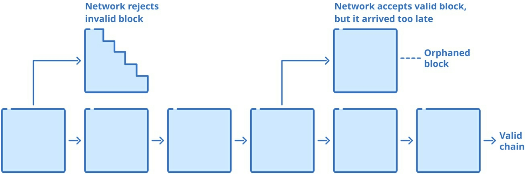
\includegraphics[width=10cm]{imagens/capitulo6/Capitulo6-Chainsplit.png}
  \caption*{\textit{\small O chain split é um processo natural que ocorre quando dois mineradores encontram blocos simultaneamente. A rede que se tornar mais pesada pela prova de trabalho se dita valida e a outra rede é feita órfão.}}
\end{figure}

%Adicionado
O bloco brasileiro agora é chamado de \textit{órfão}. Uma vez que foi rejeitado, significa que o minerador que o encontrou não foi recompensado, e as transações não entraram no livro-razão. 
Porem as transações rejeitada não estão perdidas.
Algumas dela podem ter entrado na rede japonesa competidora, e as que eventualmente não entrarão, podem ser escritos no próximo bloco.

%adicionado
Mineradores armazenam todas as transações que eles escutam num lugar especial em seus computadores chamado de como \textit{mempool}. Qualquer transação que esta no bloco que foi rejeitado é colocado de volta na mempool. Que são então minerados por alguém no futuro contanto que elas entrem em conflito a histórico do livro-razão produzido pelo bloco mais recente.

Você pode notar que, embora tenha me referido aos nodes como brasileiros e japoneses, na realidade os nodes não sabem nada sobre a identidade uns dos outros, localização geográfica e assim por diante. A única prova de validade de que precisam é que alguém tenha a cadeia de Prova de Trabalho Cumulativa Mais Longa e que as transações na cadeia sejam todas válidas (sem gastos duplos, etc.).

%modificado
A probabilidade de ocorrer essa divisão da cadeia é muito baixa - costumava acontecer uma vez por mês ou menos, mas recentemente não aconteceu muito devido a melhorias na tecnologia de propagação de bloco e conectividade de rede entre os mineradores.
Hoje e no futuro previsível, o Bitcoin tem um limite para a quantidade de informação que um bloco pode ter, definido no seu código.
Parte da razão pela qual o Bitcoin produz blocos relativamente pequenos aproximadamente a cada dez minutos é para garantir que os blocos órfãos sejam extremamente raros.
A outra razão é manter os requisitos de hardware para executar um node relativamente baixos para encorajar mais nodes no sistema.

%modificado
Mineração é probabilística. 
As vezes blocos estão a dez minutos um do outro, as vezes alguns segundos.
Se nodes produzíssemos blocos a cada segundo ou tivéssemos blocos muito grandes, teríamos uma probabilidade muito alta de que os blocos brasileiros e japoneses entrariam em conflito porque eles estão geograficamente distantes e levam mais tempo para se alcançarem. Se os órfãos acontecessem com muita frequência, a cadeia de blocos se desfaria porque haveria órfãos em órfãos e os nodes não seriam capazes de concordar sobre um histórico linear de transações antes do próximo bloco ser minerado.
%

%adicionado
É importante manter pequeno o tamanho do bloco para aumentar a chance da rede inteira possa receber o bloco mais recentes antes que um novo seja minerado.
O outro e talvez mais importante motivo, é para manter os requisitos de hardware relativamente baixos para rodar um node, encorajando mais nodes, e mineradores descentralizados a participarem da rede.
Blocos grandes encorajam a utilização de data centers e dadas regiões geográficas para minimizar blocos órfão, que impactam negativamente no lucro das operações.

\section*{A única verdadeira rede} %% seção %THE one true chain


Vamos voltar ao nosso exemplo do Capítulo 3, onde Henrique se junta a uma rede pela primeira vez.

O node do Henrique vai conectar a alguns outros node na rede e perguntar se conhecem outros nodes e depois conectar-se a eles. Esse processo é conhecido como descoberta de nodes.

Alguns desses nodes vão ser descaradamente malignos e dar a ele uma copia falsa do livro-razão, com assinaturas incorretas para transações ou com Bitcoins forjados através de mineração impropria, sem hashes de prova de trabalho validos. Essas copias serão rejeitadas de cara e esses nodes proibidos de conectar ao Henrique no futuro.

Outros nodes que ele conectar serão honestos, porem terão versões conflitantes da verdade. Por exemplo, talvez esses node tenha ficado offline e perdido a mineração de alguns blocos. Se ele baixar varias versões da blockchain e todas estão equivalentemente validas, o software no seu node vai utilizar o consenso de Nakamoto. Medindo a quantidade acumulada de prova de trabalho, qualquer das redes que tiver medido o maior valor  será  considerada a única verdadeira rede.

%adicionado
Os nodes constantemente conversam uns com os outros para garantir que tenham os blocos mais recentes.
Se o seu node quiser saber qual cópia da blockchain é verdadeira, ele só precisa procurar a cadeia com a Prova de Trabalho mais cumulativa.
Sendo assim \TraducaoNomeH{} não depende do voto da maioria, que seria fácil de trapacear utilizando uma maioria de nodes malignos

%adicionado
Mesmo que \TraducaoNomeH{} se conecte a duzias de nodes desatualizados ou malignos e apenas um node correto, o software do Bitcoin saberá qual é a copia correta devido  da quantidade de prova de trabalho acumulada e a validade das transações. A importância disso é subestimada, \TraducaoNomeH{} não depende de confiança em nenhum partida; o node vai performar todas as validações para garantir que a rede que eles ta procurando é a única verdadeira rede.

% Um node do Bitcoin precisa apenas se conectar a um outro node honesto que tenha o blockchain mais recente na rede para evitar ser enganado por invasores que podem fornecer informações falsas.
% Como todos os outros também estão seguindo esta regra, codificada no software, isso garante que haja consenso sobre qual é o verdadeiro estado do livro-razão.

É extremamente difícil, portanto, para hackers mal-intencionados fornecer a um node uma cópia falsa do blockchain, pois isso exigiria cortar a conexão desse node com qualquer outro node honesto e conectá-lo apenas a nodes malignos.




%Embora o fork normalmente aconteça devido ao acaso e atrasos de propagação de blocos, ao invés de ser motivado maliciosamente, também é possível que uma entidade sem boas intenções que deseja controlar o que vai para o próximo bloco possa tirar vantagem do Consenso de Nakamoto, controlando mais de 50\% do total do hash da rede e produzindo a mais longa cadeia de Prova de Trabalho Cumulativa. Discutiremos os detalhes desse caso, chamado de "ataque de 51\%", no Capítulo 9.


%e obtém diferentes cópias do livro-razão. O livro-razão que ele pegou da Carol é honesto, mas os livros-razão do Evandro, Danilo e Fernanda são maliciosos, onde eles excluíram um bloco antigo que continha os gastos originais da Alice para que eles pudessem enganar Henrique fazendo-o pensar que ela ainda tinha suas moedas. Antes de vincular os blocos entre si por Prova de Trabalho, Henrique não sabia que um bloco antigo foi excluído.


\begin{figure}
  \centering
  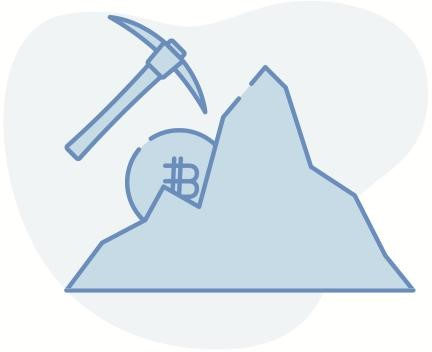
\includegraphics[width=5cm]{imagens/capitulo-06-mineracao.jpg}
  \caption*{\textit{\small Ao contrário da mineração de ouro, que também consome energia, o processo de mineração de Bitcoin na verdade protege a rede para tornar o livro-razão à prova de adulteração.}}
\end{figure}




%seção adicionada
\section*{Reversibilidade das transações}

%modificado
Duas redes competindo normalmente são produzidas ao acaso e resolvidas rapidamente.
Porem uma pessoa que deseja atacar a rede bitcoin pode se aproveitar do consenso de Nakamoto controlando mais do que 50\% da taxa de hash total.
Assim eles produziriam a rede com prova de trabalho acumulado mais longa, que poderia conter transações de suas escolhas contanto que ele estejam dispostos a gastar a energia para tal. 
Quando eles publicarem nessa cadeia, os outros nos da rede aceitariam ele como o única verdadeira rede. 
Isso é conhecido como ataque de 51\% porque requer o controle centralizado de  mais da metade da rede.

%parcialmente adicionado
É importante entender que não há finalidade real de transação no Bitcoin, visto que ataques de 51\% ou a chance de criar blocos órfãos são sempre teoricamente possíveis.
Por conta disso, recipientes de transações tipicamente esperam algumas blocos serem minerados sobre a transação para considerar ela escrita em pedra.
Nesse ponto, a quantidade de energia requerida para reverter a transação é tao cara, que ela provavelmente não vai acontecer.

%parcialmente adicionado
Blocos minerados apos um bloco contendo uma transação de interesse a você normalmente são chamados de confirmações, então quando ouvires que uma dada transação possui seis confirmações isso quer dizer que foram minerados seis blocos depois da transação. 
Se você está vendendo um livro digital que tem custo marginal para você como comerciante, pode querer apenas 1 confirmação, ou mesmo zero confirmações, entregando o bem digital assim que vir a transmissão da transação na rede. 
Se você está vendendo uma casa, talvez queira esperar por doze confirmações, ou cerca de duas horas de mineração.
Quanto mais você espera, mais Provas de Trabalho são empilhadas no topo do bloco que contém suas transações e mais caro se torna no mundo real para reverter a transação.
Cada comerciante ou processador de pagamentos decide por si mesmo o que considera final. 
Hoje, a maioria das pessoas aceita 6 confirmações - seis blocos extraídos depois daquele que contém a transação - como sendo definitivo, mas os comerciantes podem definir isso como quiserem.

Se a taxa de hash do Bitcoin cair significativamente, o que significa que menos energia está protegendo cada bloco, pode-se sempre aumentar o número de confirmações necessárias para a liquidação final.
Embora isso possa parecer muito complicado no início, é importante ter em mente que as transações com cartão de crédito normalmente podem ser revertidas 120 dias após serem feitas.

%modificado
Por outro lado, o Bitcoin é um dinheiro de liquidação final que não pode ser retirado de você, como dinheiro ou ouro. Deste ponto de vista, a reversibilidade e a finalidade das transações no Bitcoin é, na verdade, uma vasta melhoria em relação à maioria das redes de pagamento tradicionais.

%adicionado
A estimativas de hoje mostram que se tivesse toda a energia da rede Bitcoin ao seu dispor - o que é uma presunção e tanto, visto que terias ao que ter ao seu dispor a energia de um pais, e todas as equipamentos especializados do mundo - ainda seria necessário mais de um ano de mineração para reescrever a histórico de transações da rede. É possível ver tais dados em \url{http://bitcoin.sipa.be/}


Em um mercado em queda, o ciclo pode ir na outra direção, com os usuários vendendo as moedas, fazendo com que o preço caia e os mineiros se tornem não lucrativos. No entanto, ao contrário do que se pode ler na mídia sobre uma “espiral da morte”, o algoritmo de ajuste de dificuldade garante que sempre haverá algum tipo de equilíbrio entre o preço e o número de mineradores na rede. Também retira os mineradores ineficientes em favor dos que operam com a energia mais barata possível.